% Drawing 138/04-8 -- folder 138, batch 04, archive page 77 (PDF page 78).
% Transcription: en bas, une sphère avec un parallèle, puis un cercle coupant une droite graduée $-1$, $0$, $\frac{1}{2}$, $1$, $2$, les arcs passant par un point marqué $j$ au-dessus et $\bar{j}$ au-dessous de l'axe (signes douteux) ; à gauche, $\mathbb{P}^{1}_{\mathbb{Q}} \xleftarrow{\ \varphi\ } \mathbb{P}^{1}_{\mathbb{Q}}$.
% Kind: sphere with a parallel; circles over a graduated line. Method 2 (schematic redraw from the facsimile). Status: partial.
% Notes: Pencil. Left: a sphere (outline broken at the lower left, as on the page) with a tilted parallel and a meridian from the top point to the bottom point through the upper point of the parallel; the points at the top, the bottom, both ends of the parallel and on the meridian are marked. Right: a graduated line with ticks at -1, 0, 1/2, 1, 2 (each tick computed on the line), a near-vertical line through 1/2, a large closed curve through -1 and 2 and an oval through 0 and 1; both pass through the point marked -j above the axis and the point marked -j-bar below it, where his curves meet (every curve drawn through the same two points). Labels as on the page: « -j » and « -j-bar », with a minus sign, where the transcription has j and j-bar (« signes douteux »); the label at 1/2 looks like « h » on the page and is set as 1/2 after the transcription. At the left, P^1_Q <-phi- P^1_Q. The bbox is widened to the right so that the tick 2 and the right side of the large curve are inside. Still differs: his doubled pencil strokes (the right side of the sphere, the lower arcs of both curves) are drawn once; the curves are traced through points read off the crop, about one unit off in places. Left out: the strokes at the top right, which belong to the pentagon tiling (04-7). Nothing is struck. Redrawn 2026-11-09 (issue 128): to check again.
% Coordinates: 1 unit = 1 mm = 1/100 of the crop width (bbox in page fractions: [0.08, 0.47, 0.72, 0.78]).
% Redrawn by Claude (claude-opus-5-5), issue #73, 2026-11-09; not checked by a human; not compiled (no TeX in the session).
% Rights: reproduces part of the work -- behind RENDER_TRANSCRIPTS, never published by itself.
\documentclass[tikz,border=3pt]{standalone}
\usepackage{amsmath,amssymb}
\usetikzlibrary{patterns,arrows.meta}
\tikzset{pencil/.style={black!45}, struck/.style={black!35}, mark/.style={circle,draw,inner sep=1.3pt}, pt/.style={circle,fill,inner sep=0.9pt}, opt/.style={circle,draw,fill=white,inner sep=1.1pt}}
\begin{document}
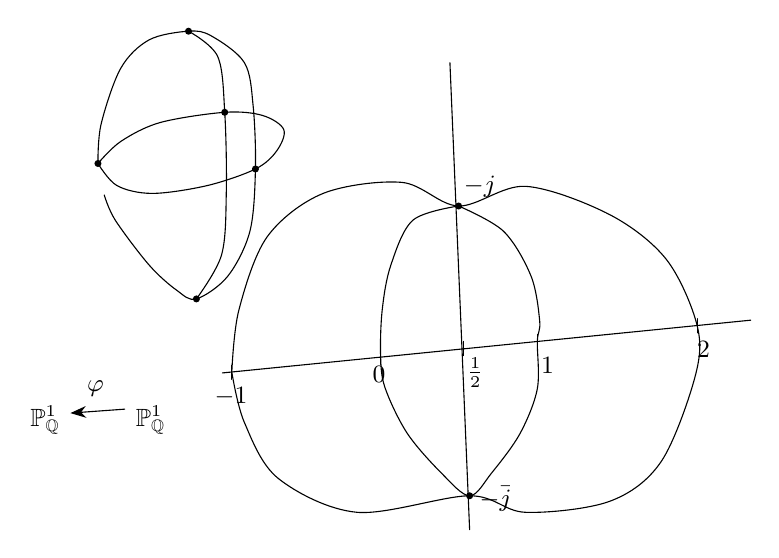
\begin{tikzpicture}[x=1mm,y=1mm,line cap=round,line join=round,font=\scriptsize]
\draw plot[smooth, tension=0.55] coordinates {(17.9,-25.4) (19.3,-28.6) (23.6,-34.3) (27.1,-37.5) (29.6,-38.6) (33.6,-35.7) (36.4,-30) (37.1,-22.1) (36.8,-14) (35.7,-8.6) (31.5,-5.2) (28.6,-4.6) (23.6,-5.7) (20,-9.3) (17.5,-16.4) (17.1,-21.4)};
\draw plot[smooth, tension=0.55] coordinates {(17.1,-21.4) (20,-18.6) (25,-16.2) (33.2,-14.9) (38,-15.3) (40.7,-17.1) (39.8,-19.8) (37.1,-22.1) (31,-24.2) (24,-25.2) (19.5,-24.2) (17.1,-21.4)};
\draw plot[smooth, tension=0.55] coordinates {(28.6,-4.6) (32.3,-7.8) (33.2,-14.9) (33.4,-25) (32.8,-33) (29.6,-38.6)};
\node[pt] at (17.1,-21.4) {};
\node[pt] at (33.2,-14.9) {};
\node[pt] at (37.1,-22.1) {};
\node[pt] at (28.6,-4.6) {};
\node[pt] at (29.6,-38.6) {};
\draw (32.9,-48) -- (100,-41.3);
\draw (34.1,-47) -- (34.1,-48.8);
\draw (53,-45.1) -- (53,-46.9);
\draw (63.5,-44) -- (63.5,-45.8);
\draw (72.9,-43.1) -- (72.9,-44.9);
\draw (93.2,-41.1) -- (93.2,-42.9);
\draw (61.8,-8.6) -- (64.3,-67.9);
\draw plot[smooth, tension=0.55] coordinates {(34.1,-47.9) (35,-40) (38.6,-30.7) (45.7,-25.2) (55.7,-23.8) (62.9,-26.8) (71.4,-24.3) (82.1,-27.9) (89.3,-33.6) (93.2,-42) (92.9,-48.6) (88.6,-59.3) (82.1,-64.3) (71.4,-65.7) (64.3,-63.6) (50,-65.7) (40,-61.4) (35.7,-54.3) (34.1,-47.9)};
\draw plot[smooth, tension=0.55] coordinates {(62.9,-26.8) (57.1,-28.6) (54.3,-34.3) (53.2,-40) (53,-46) (53.6,-50) (56.4,-55.7) (60.7,-60.7) (64.3,-63.6) (67.1,-60.7) (70.7,-55.7) (72.9,-50) (72.9,-44) (73.2,-41.4) (72.1,-35.7) (68.6,-30) (62.9,-26.8)};
\node[pt] at (62.9,-26.8) {};
\node[pt] at (64.3,-63.6) {};
\node[inner sep=1pt] at (34,-51) {\small $-1$};
\node[inner sep=1pt] at (52.8,-48.2) {\small $0$};
\node[inner sep=1pt] at (65,-48) {\small $\frac12$};
\node[inner sep=1pt] at (74.2,-47) {\small $1$};
\node[inner sep=1pt] at (94,-45) {\small $2$};
\node[inner sep=1pt] at (65.6,-24.4) {\small $-j$};
\node[inner sep=1pt] at (67.6,-64) {\small $-\bar j$};
\node[inner sep=1pt] at (10.4,-54) {\small $\mathbb{P}^1_{\mathbb{Q}}$};
\draw[-{Stealth[length=2mm]}] (20.5,-52.6) -- (13.6,-53.1);
\node[inner sep=1pt] at (16.8,-50) {\small $\varphi$};
\node[inner sep=1pt] at (23.8,-54) {\small $\mathbb{P}^1_{\mathbb{Q}}$};
\end{tikzpicture}
\end{document}
